\documentclass{exam}

\usepackage{fullpage}
\usepackage{enumerate}
\usepackage{siunitx} 
\usepackage{graphicx}
\usepackage[fleqn]{amsmath}
\usepackage{cancel}
\usepackage{polynom}
\usepackage{float}
\usepackage{mdwlist}
\usepackage{booktabs}
\usepackage{cancel}
\usepackage{polynom}
\usepackage{caption}

\newcommand{\degree}{\ensuremath{^\circ}} 
\everymath{\displaystyle}

% \begin{figure}[H]
%   \centering
%   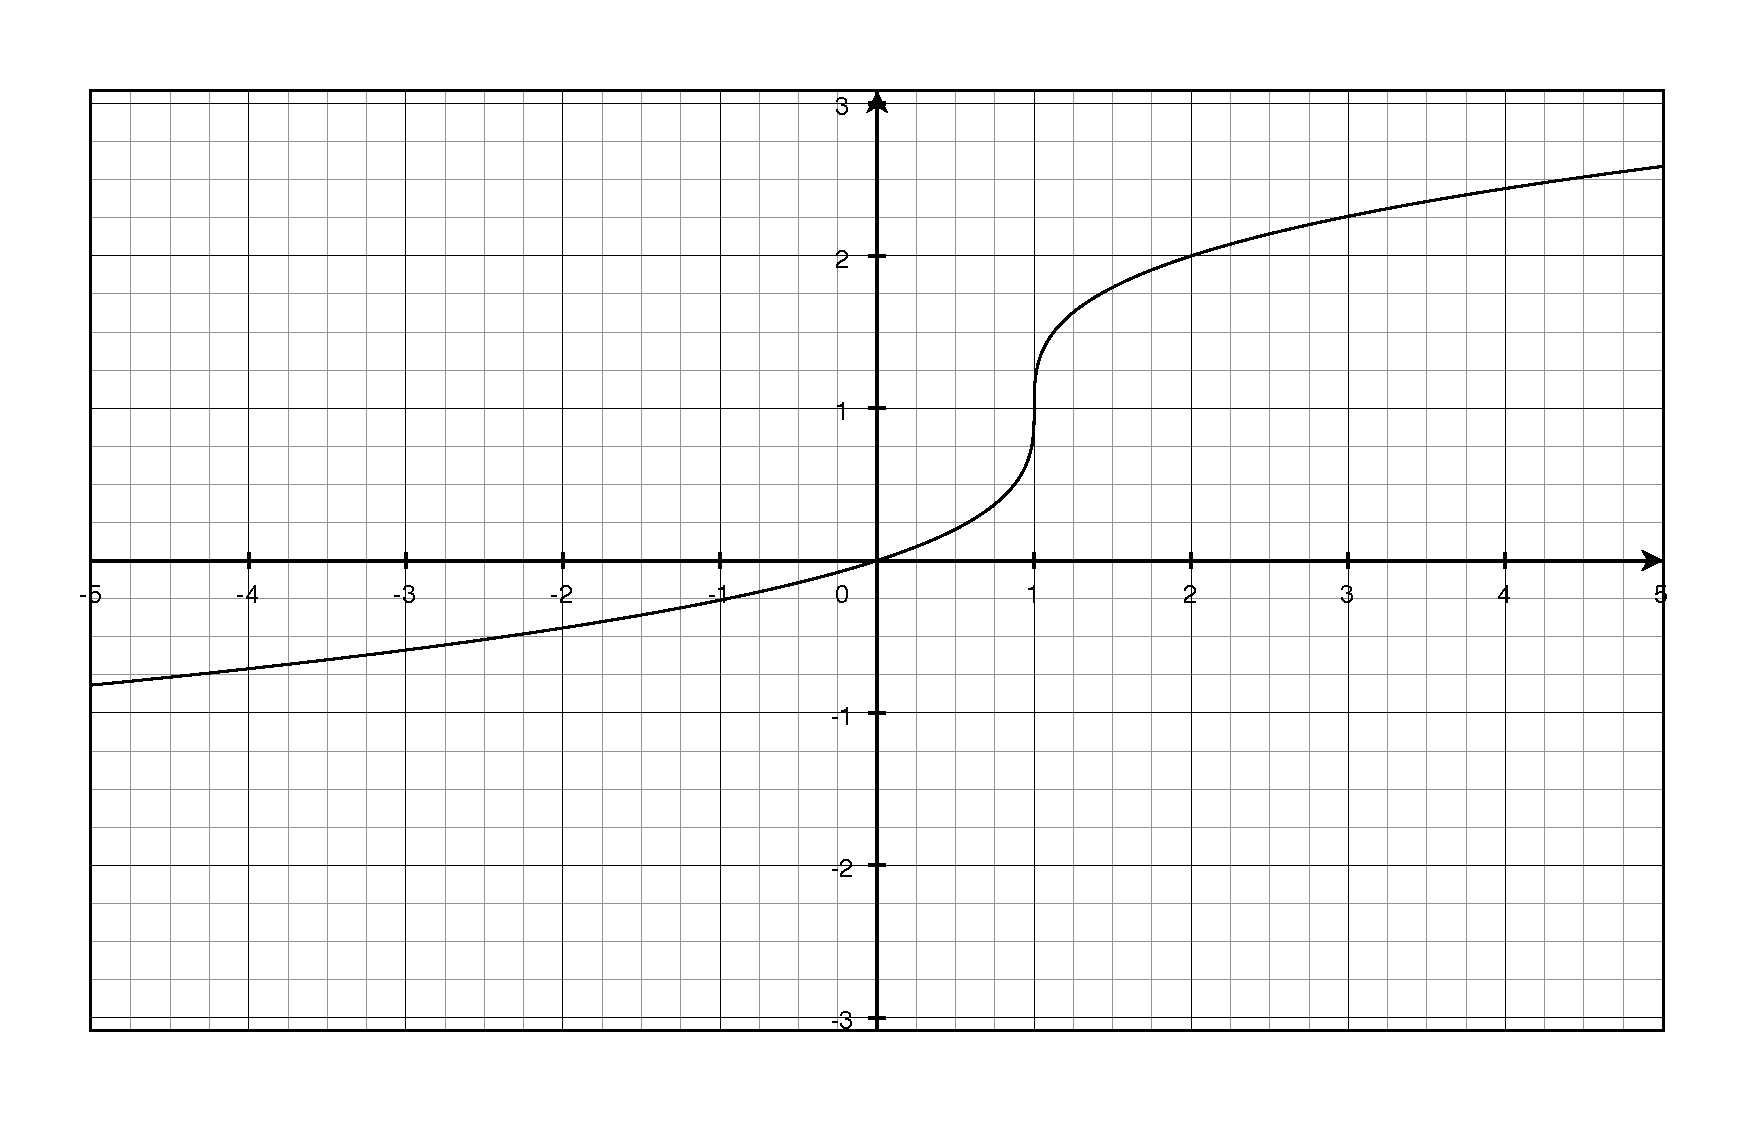
\includegraphics[scale=.3]{question7.eps}
%   \caption*{Question 7}
% \end{figure}

% \begin{tabular}{cc}
% \toprule
% period & amplitude \\
% \midrule
%   $\pi$ & $2$ \\
% \bottomrule
% \end{tabular}

\printanswers

\ifprintanswers 
\usepackage{2in1, lscape} 
\fi

\title{Math 263a \\ Homework Seven}
\date{March 7, 2012}

\begin{document}

\maketitle

\section{Homework}

\begin{itemize*}
  \item Read Section 3.4-3.5
  \item pp. 121-122: 28-32 (I accidentally forgot to include the product rule questions last week)
  \item pp. 127-128: 1-12, 17-18, 24
  \item pp. 132-133: 1-5, 11-15, 21-25, 27-28, 41-45
\end{itemize*}

\section{Extra Credit}
Page 133, problem 50

\ifprintanswers

\begin{enumerate}[a]

\item
The point is on the unit circle and the angle is changing at the rate of $\theta = 2t$, so the coordinates are
$(\cos(2t), \sin(2t))$

\item
\begin{itemize*}
  \item The horizontal side of the triangle with the connecting rod as the hypotenuse is $\cos(2t)$.  
  \item The vertical side of this triangle is $\sqrt{25 - \cos^2(2t)}$
\end{itemize*}

The y-coordinate is the length of the vertical side plus the y coordinate of P, or:
\[
  y = \sin(2t) + \sqrt{25 - \cos^2(2t)}
\]

\item
The velocity is the derivative of the y-coordinate:
\begin{align*}
  y &= \sin(2t) + \sqrt{25 - \cos^2(2t)} \\
  v &= 2 \cos(2t) + \frac{1}{2} (25 - cos^2(2t))^{-1/2} \cdot (-2 \cos(2t)) \cdot (- \sin(2t)) \cdot 2 \\
    &= 2 \cos(2t) + \frac{2 \cos(2t) \sin(2t)} {\sqrt{25 - cos^2(2t)}} \\
    &= 2 \cos(2t) \left(1 + \frac{\sin(2t)} {\sqrt{25 - cos^2(2t)}} \right) \\
\end{align*}
\end{enumerate}

You can see in the graph that the velocity is zero when the the piston is turning around at the top or bottom of its
stroke.

\begin{figure}[H]
  \centering
  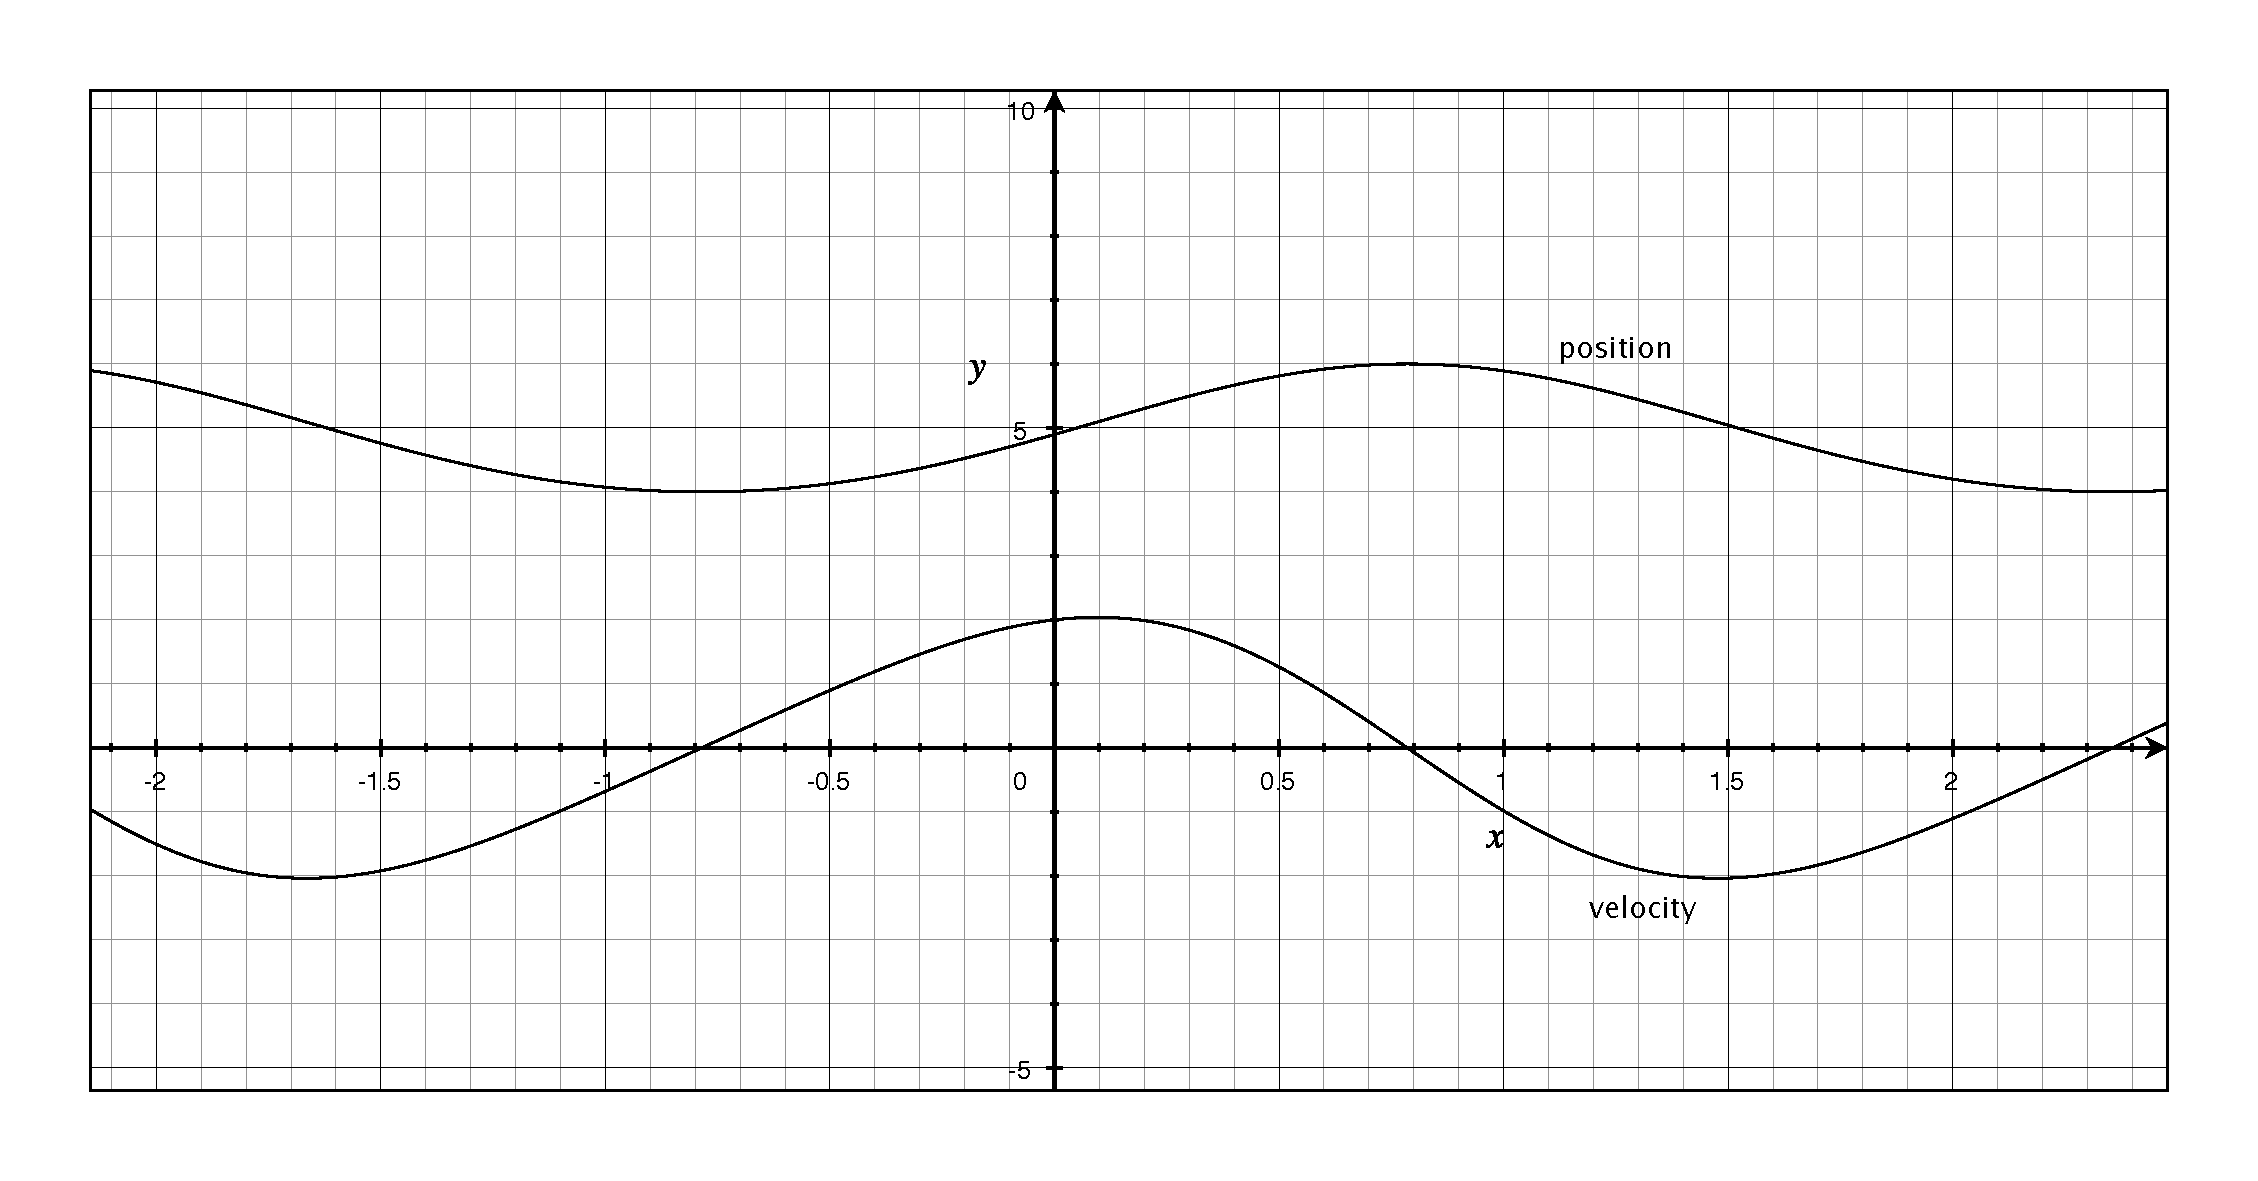
\includegraphics[scale=.3]{extra_credit.eps}
  \caption*{Extra Credit}
\end{figure}

\section{Homework}

\subsection{Section 3.3}

\begin{description}
\item[28]
\begin{align*}
  y &= (x^4 - 1)(x^2 + 1) \\
  y'&= (x^4 - 1)(2x) + (4x^3)(x^2 + 1) \\
    &= 2x^5 - 2x + 4x^5 + 4x^3 \\
    &= 6x^5 + 4x^3 - 2x \\
\end{align*}

\item[29]
\begin{align*}
  y &= (x^2 + 17)(x^3 - 3x + 1) \\
  y'&= (x^2 + 17)(3x^2 - 3) + (2x)(x^3 - 3x + 1) \\
    &= 3x^4 - 3x^2 + 51x^2 - 51 + 2x^4 - 6x^2 + 2x \\
    &= 5x^4 + 42x^2 + 2x - 51 \\
\end{align*}

\item[30]
\begin{align*}
  y &= (x^4 + 2x)(x^3 + 2x^2 + 1) \\
  y'&= (x^4 + 2x)(3x^2 + 4x) + (4x^3 + 2)(x^3 + 2x^2 + 1) \\
    &= 3x^6 + 4x^5 + 6x^3 + 8x^2 + 4x^6 + 8x^5 + 4x^3 + 2x^3 + 4x^2 + 2 \\
    &= 7x^6 + 12x^5 + 12x^3 + 12x^2 + 2 \\
\end{align*}

\item[31]
\begin{align*}
  y &= (5x^2 - 7)(3x^2 - 2x + 1) \\
  y'&= (5x^2 - 7)(6x - 2) + (10x)(3x^2 - 2x + 1) \\
    &= 30x^3 - 10x^2 - 42x + 14 + 30x^3 - 20x^2 + 10x \\
    &= 60x^3 - 30x^2 - 32x + 14 \\
\end{align*}

\item[32]
\begin{align*}
  y &= (3x^2 + 2x)(x^4 - 3x + 1) \\
  y'&= (3x^2 + 2x)(4x^3 - 3) + (x^4 - 3x + 1)(6x + 2) \\
    &= (12x^5 - 9x^2 + 8x^4 - 6x) + (6x^5 - 18x^2 + 6x + 2x^4 - 6x + 2) \\
    &= (12x^5 + 8x^4 - 9x^2 - 6x) + (6x^5 + 2x^4 - 18x^2 + 2) \\
    &= 18x^5 + 10x^4 - 27x^2 - 6x + 2 \\
\end{align*}

\end{description}

\subsection{Section 3.4}

\begin{description}

\item[1]
\begin{align*}
  y  &= 2 \sin x + 3 \cos x \\
  y' &= 2 \cos x - 3 \sin x \\ 
\end{align*}

\item[2]
\begin{align*}
  y  &= \sin^2 x \\
  y' &= 2 \sin x \cos x \\ 
\end{align*}

\item[3]
\begin{align*}
  y  &= \sin^2 x + \cos^2 x = 1 \\
  y' &= 0 \\ 
\end{align*}

\item[4]
\begin{align*}
  y  &= 1 - \cos^2 x = \sin^2 x \\
  y' &= 2 \sin x \cos x \\ 
\end{align*}

\item[5]
\begin{align*}
  y  &= \sec x = \frac{1}{\cos x} \\
  y' &= \frac{\sin x}{\cos^2 x} \\ 
     &= \tan x \sec x \\
\end{align*}

\item[6]
\begin{align*}
  y  &= \csc x = \frac{1}{\sin x} \\
  y' &= \frac{- \cos x}{\sin^2 x} \\ 
     &= - \cot x \csc x \\
\end{align*}

\item[7]
\begin{align*}
  y  &= \tan x = \frac{\sin x}{\cos x} \\
  y' &= \frac{\cos x \cos x - \sin x (-\sin x)}{\cos^2 x} \\ 
     &= \frac{\cos^2 x + \sin^2 x}{\cos^2 x} \\ 
     &= \frac{1}{\cos^2 x} \\ 
     &= \sec^2 x \\
\end{align*}

\item[8]
\begin{align*}
  y  &= \cot x = \frac{\cos x}{\sin x} \\
  y' &= \frac{\sin x(- \sin x) - (\cos x) (\cos x)}{\sin^2 x} \\ 
     &= \frac{- (\sin^2 x + \cos^2 x)}{\sin^2 x} \\ 
     &= - \frac{1}{\sin^2 x} \\ 
     &= - \csc^2 x \\
\end{align*}

\item[9]
\begin{align*}
  y  &= \frac{\sin x + \cos x}{\cos x} \\
     &= \tan x + 1 \\
  y' &= \sec^2 x \text{ from problem 7} \\
\end{align*}

\item[10]
\begin{align*}
  y  &= \frac{\sin x + \cos x}{\tan x} \\
  y' &= \frac{(\tan x)(\cos x - \sin x) - (\sin x + \cos x)(\sec^2 x)}{\tan^2 x}  \\
     &= \frac{\frac{\sin x}{\cos x}(\cos x - \sin x) - \frac{1}{\cos^2 x}(\sin x + \cos x)}{\tan^2 x}  \\
     &= \frac{\sin x - \sin x \tan x - \sin x \tan x - \sec x)}{\tan^2 x}  \\
     &= \frac{\sin x - 2 \sin x \tan x - \sec x)}{\tan^2 x}  \\
\end{align*}

\item[11]
\begin{align*}
  y  &= x^2 \cos x \\
     &= - x^2 \sin x + 2x \cos x \\
\end{align*}

\item[12]
\begin{align*}
  y  &= \frac{x \cos x + \sin x}{x^2 + 1} \\
     % &= \frac{(x^2 + 1)(D_x (x \cos x + \sin x)) - (x \cos x + \sin x)(2x)}{(x^2 + 1)^2} \\
     &= \frac{(x^2 + 1)(- x \sin x + \cos x + \cos x) - (2x^2 \cos x + 2x \sin x)}{(x^2 + 1)^2} \\
     &= \frac{(x^2 + 1)(- x \sin x + 2\cos x) - 2x^2 \cos x - 2x \sin x)}{(x^2 + 1)^2} \\
     &= \frac{-x^3 \sin x + 2 x^2 \cos x - x\sin x + 2 \cos x - 2x^2 \cos x - 2x \sin x}{(x^2 + 1)^2} \\
     &= \frac{-x^3 \sin x - 3x\sin x + 2 \cos x}{(x^2 + 1)^2} \\
\end{align*}

\item[17]
\begin{align*}
  \lim_{x \to 0} \frac{\sin x}{2x} &= \frac{1}{2} \lim_{x \to 0} \frac{\sin x}{x} \\
    &= \frac{1}{2}  \\
\end{align*}

\item[18]
\begin{align*}
  \lim_{x \to 0} \frac{\sin 3 \theta}{2 \theta} &= \frac{3}{2} \lim_{x \to 0} \frac{\sin 3 \theta}{3 \theta} \\
    &= \frac{3}{2}  \\
\end{align*}

\item[24]

The height is given by:
\[
  y = 2 \sin t
\]
The velocity is the derivative of the position:
\[
  v = 2 \cos t \\
\]

The volocity at the indicated times is:

\begin{tabular}{cc}
\toprule
t (s) & v (cm/s)\\
\midrule
0               &  2 \\
$\frac{\pi}{2}$ &  0 \\
$\pi$           & -2 \\
\bottomrule
\end{tabular}

\end{description}

\subsection{Section 3.5}

\begin{description}

\item[1]
\begin{align*}
  y  &= (1+x)^{15} \\
  y' &= 15(1+x)^{14} \\
\end{align*}

\item[2]
\begin{align*}
  y  &= (7 + x)^5\\
  y' &= 5 (7+x)^4\\
\end{align*}

\item[3]
\begin{align*}
  y  &= (3 - 2x)^5 \\
  y' &= 5 (3 - 2x)^4 (-2) \\
     &= -10 (3 - 2x)^4 \\
\end{align*}

\item[4]
\begin{align*}
  y  &= (4 + 2x^2)^7\\
  y' &= 7 (4 + 2x^2)^6 (4x) \\
     &= 28x (4 + 2x^2)^6 \\
\end{align*}

\item[5]
\begin{align*}
  y  &= (x^3 - 2x^2 + 3x + 1)^{11} \\
  y' &= 11 (x^3 - 2x^2 + 3x + 1)^{10} (3x^2 - 4x + 3) \\
\end{align*}

\item[11]
\begin{align*}
  y  &= \sin(x^2 + x) \\
  y' &= \cos(x^2 + x) \cdot (2x + 1)\\
\end{align*}

\item[12]
\begin{align*}
  y  &= \cos(3x^2 - 2x)\\
  y' &= - \sin(3x^2 - 2x) \cdot (6x - 2) \\
\end{align*}

\item[13]
\begin{align*}
  y  &= [ \cos x]^3 \\
  y' &= 3 \cos^2 x \cdot (- \sin x) \\
     &= -3 \cos^2 x \sin x \\
\end{align*}

\item[14]
\begin{align*}
  y  &= \sin^4(3x^2) = [\sin(3x^2)]^4 \\
  y' &= 4 [\sin (3x^2)]^3 \cdot \cos(3x^2) \cdot 6x \\
     &= 24x \sin^3(3x^2) \cos(3x^2) \\
\end{align*}

\item[15]
\begin{align*}
  y  &= \left( \frac{x+1}{x-1} \right)^3 \\
  y' &= 3 \left( \frac{x+1}{x-1} \right)^2 \left( \frac{x-1 - (x + 1)}{(x-1)^2} \right) \\
     &= 3 \cdot \frac{(x+1)^2}{(x-1)^2} \cdot \frac{-2}{(x-1)^2} \\
     &= \frac{-6 (x+1)^2}{(x-1)^4} \\
\end{align*}

\item[21]
\begin{align*}
  y  &= (3x - 2)^2 (3 - x^2)^2 \\
  y' &= (3x - 2)^2 (2)(3 - x^2)(-2x) + (2)(3x - 2)(3)(3-x^2)^2 \\
     &= -4x (3x - 2)^2(3 - x^2) + 6(3x - 2)(3-x^2)^2 \\
     &= 2(3x-2)(3-x^2) [-2x (3x - 2) + 3(3-x^2) ] \\
     &= 2(3x-2)(3-x^2)(-6x^2 + 4x + 9 - 3x^2) \\
     &= 2(3x-2)(3-x^2)(-9x^2 + 4x + 9) \\
\end{align*}

\item[22]
\begin{align*}
  y  &= (2 - 3x^2)^4(x^7 + 3)^3 \\
  y' &= (2 - 3x^2)^4 \cdot 3(x^7 + 3)^2(7x^6) +  (x^7 + 3)^3 \cdot 4(2 - 3x^2)^3(-6x) \\
     &= 21x^6 (2 - 3x^2)^4(x^7 + 3)^2 - 24x (x^7 + 3)^3(2 - 3x^2)^3 \\
     &= (2 - 3x^2)^3 (x^7 + 3)^2 (- 87x^8 + 42 x^6  - 72x) \\
\end{align*}

\item[23]
\begin{align*}
  y  &= \frac{(x+1)^2}{3x-4} \\
  y' &= \frac{(3x-4)(2)(x+1) - (x+1)^2(3)}{(3x - 4)^2} \\
     &= \frac{6x^2 - 2x - 8 - 3x^2 - 6x -3}{(3x - 4)^2} \\
     &= \frac{3x^2 - 8x - 11}{(3x - 4)^2} \\
\end{align*}

\item[24]
\begin{align*}
  y  &= \frac{2x - 3}{(x^2 + 4)^2} \\
  y' &= \frac{ (x^2 + 4)^2(2) - (2x - 3)(2)(x^2 + 4)(2x) }{(x^2 + 4)^4}  \\
     &= \frac{ 2(x^2 + 4)^2 - 4x(2x - 3)(x^2 + 4) }{(x^2 + 4)^4}  \\
     &= \frac{ 2(x^2 + 4) - 4x(2x - 3) }{(x^2 + 4)^3}  \\
     &= \frac{ 2x^2 + 8 - 8x^2 + 12x }{(x^2 + 4)^3}  \\
     &= \frac{ -6x^2 + 12x + 8 }{(x^2 + 4)^3}  \\
\end{align*}

\item[25]
\begin{align*}
  y  &= \frac{(3x^2 + 2)^2}{2x^2 - 5} \\
  y' &= \frac{(2x^2 - 5) \cdot 2(3x^2 + 2)(6x) -(3x^2 + 2)^2(4x) } {(2x^2 - 5)^2} \\
     &= \frac{12x (2x^2 - 5)(3x^2 + 2) - 4x(3x^2 + 2)^2 } {(2x^2 - 5)^2} \\
     &= \frac{4x(3x^2 + 2) [ 3(2x^2 - 5) - (3x^2 + 2)] } {(2x^2 - 5)^2} \\
     &= \frac{4x(3x^2 + 2) [ 6x^2 - 15 - 3x^2 - 2)] } {(2x^2 - 5)^2} \\
     &= \frac{4x(3x^2 + 2) (3x^2 - 17) } {(2x^2 - 5)^2} \\
\end{align*}

%% \item[26]
%% \begin{align*}
%%   y  &= \frac{(x^2 - 1)^3}{(4x^3 - 5)^2} \\
%%   y' &= \frac{(4x^3 - 5)^2 \cdot 3(x^2 - 1)^2(2x) - (x^2 - 1)^3 \cdot 2(4x^3 - 5)(12x^2) } {(4x^3 - 5)^4 } \\
%%      &= \frac{6x (4x^3 - 5)(x^2 - 1)^2 - 24x^2 (x^2 - 1)^3} {(4x^3 - 5)^3 } \\
%%      &= \frac{6x(x^2 - 1)^2[ (4x^3 - 5) - 4x(x^2 - 1)]} {(4x^3 - 5)^3 } \\
%%      &= \frac{6x(x^2 - 1)^2(4x^3 - 5 - 4x^3 + 4x)} {(4x^3 - 5)^3 } \\
%%      &= \frac{6x(x^2 - 1)^2(4x - 5)} {(4x^3 - 5)^3 } \\
%% \end{align*}

\item[27]
\begin{align*}
  y  &= \left( \frac{3t - 2}{t + 5} \right)^3 \\
  y' &= 3 \left( \frac{3t - 2}{t + 5} \right)^2 \cdot \frac{(t + 5)(3) - (3t - 2)}{(t+5)^2}  \\
     &= \frac{3(3t - 2)^2}{(t + 5)^2} \cdot \frac{3t + 15 - 3t + 2)}{(t+5)^2}  \\
     &= \frac{3(3t - 2)^2}{(t + 5)^2} \cdot \frac{17}{(t+5)^2} \\
     &= \frac{51(3t - 2)^2}{(t + 5)^4} \\
\end{align*}

\item[28]
\begin{align*}
  y  &= \frac{s^2 - 9}{s + 4} \\
  y' &= \frac{(s+4)(2s) - (s^2 - 9)}{(s + 4)^2} \\
     &= \frac{2s^2 + 8s - s^2 + 9}{(s + 4)^2} \\
     &= \frac{s^2 + 8s + 9}{(s + 4)^2} \\
\end{align*}

\item[41]
\begin{align*}
  y  &= [ \sin(\cos t) ]^3 \\
  y' &= 3 [ \sin (\cos t) ]^2 \cdot \cos (\cos t) \cdot (- \sin t) \\
     &= -3 \sin^2(\cos t) \cdot \cos (\cos t) \cdot \sin t \\
\end{align*}

\item[42]
\begin{align*}
  y  &= \left[ \cos \left( \frac{u+1}{u-1} \right) \right]^4 \\
  y' &= 4 \left[ \cos \left( \frac{u+1}{u-1} \right) \right]^3 \cdot \left[ -\sin \left( \frac{u+1}{u-1} \right) \right] 
        \cdot \left[ \frac{(u-1) - (u+1)}{(u-1)^2} \right] \\
     &= 4 \cos^3 \left( \frac{u+1}{u-1} \right) \cdot \sin \left( \frac{u+1}{u-1} \right) \cdot \frac{2}{(u-1)^2} \\
\end{align*}

\item[43]
\begin{align*}
  y  &= [ \cos(\sin \theta^2 ) ]^4 \\
  y' &= 4 [ \cos(\sin \theta^2 ) ]^3 \cdot [ -\sin(\sin \theta^2 ) ] \cdot [ \cos \theta^2 ] \cdot [2 \theta ] \\
     &= -8 \theta \cdot \cos^3(\sin \theta^2) \cdot \sin(\sin \theta^2 ) \cdot \cos \theta^2 \\
\end{align*}

\item[44]
\begin{align*}
  y  &= x [\sin 2x ]^2 \\
  y' &= x \cdot 2 \sin 2x \cos 2x \cdot 2 + \sin^2 2x \cdot 1 \\
     &= 4x \sin 2x \cos 2x + \sin^2 2x \\
\end{align*}

\item[45]
\begin{align*}
  y  &= \sin [ \cos ( \sin 2x ) ] \\
  y' &= \cos [ \cos ( \sin 2x ) ] \cdot [-\sin ( \sin 2x ) ] \cdot [ \cos 2x ] \cdot 2 \\
     &= -2 \cos [ \cos ( \sin 2x ) ] \cdot \sin ( \sin 2x ) \cdot \cos 2x \\
\end{align*}



\end{description}

\else

\vspace{10 cm}

{\em People like us, who believe in physics, know that the distinction between past, present, and future is only a
  stubbornly persistent illusion.}

\vspace{.2 cm}

\hspace{1 cm} --Albert Einstein

% for approximation {\em From this point forth we shall be leaving the firm foundation of fact and journeying together
% through the murcky marshes of memory into thickets of wildest guesswork.} (Dumbledore)(Can be used right in front of
% the Humphrey Belcher quote if desired. From page 197. Humphrey Belcher quote is also from page 197. Harry Potter and
% the Half-Blood Prince. I love typing on this thing.

\fi

\end{document}

